\chapter{Current progress}

\label{ch:progress}

\section{\NP{} as puzzles, or one-move games}

Recall that \NP{} is the class of problems solvable by guess-and-check, with a
\emph{check} problem in \P{} (\cref{defn:np}):
\[
  \NP = \SetBuilder{L}{
    ∃\underbrace{\mathstrut L'∈\P}_{\mathclap{\text{the ``check'' problem}}} \;
    ∀x \quad
    x∈L ⟺ \underbrace{∃g \; (x, g) ∈ L'}_{\mathclap{\text{guess-and-check}}}
  }.
\]
(In the above, it is \emph{implicitly} required that \(\Abs g\) be
polynomially-bounded with respect to \(\Abs x\), but we have omitted it in
notation for readability.)

Another famous example of a problem in \NP{} is Sudoku, framed as the following
decision problem:
\begin{definition}[\Problem{sudoku}]%
  We are given a square grid with dimensions \(n^2\times n^2\), some of whose
  cells are filled in with numbers in \(\{1,\dotsc,n^2\}\).  Call this grid the
  Sudoku \emph{board}.  The board is evenly partitioned into \(n\) chunks along
  each axis, resulting in \(n^2\) \emph{blocks} each with dimensions \(n\times
  n\).

  Does there exist a way to fill in the rest of the cells so that each row,
  column, and block on the filled-in board contains each number in
  \(\{1,\dotsc,n^2\}\) exactly once?
\end{definition}

\begin{center}
  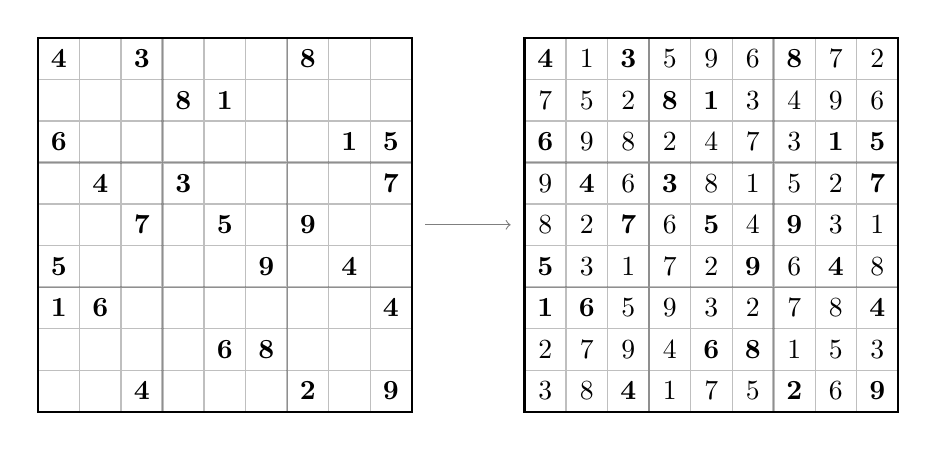
\begin{tikzpicture}[x=3em/2, y=3em/2]
    \tikzset{
      sudoku/.pic={
        \draw[thick] (0,0) rectangle (9,-9);
        \draw[thick, opacity=1/4]
        foreach \i in {3,6} { (0,-\i) -- +(9,0) (\i,0) -- +(0,-9) };
        \draw[opacity=1/4]
        foreach \i in {1,...,8} { (0,-\i) -- +(9,0) (\i,0) -- +(0,-9) };

        \path
        foreach \i in {0,...,8} { foreach \j in {0,...,8} {
            (\j+1/2,-\i-1/2) coordinate(#1-\i-\j)
        } }
        foreach \i/\j/\val in {
          0/0/4,0/2/3,0/6/8,
          1/3/8,1/4/1,
          2/0/6,2/7/1,2/8/5,
          3/1/4,3/3/3,3/8/7,
          4/2/7,4/4/5,4/6/9,
          5/0/5,5/5/9,5/7/4,
          6/0/1,6/1/6,6/8/4,
          7/4/6,7/5/8,
          8/2/4,8/6/2,8/8/9
        } { (#1-\i-\j) node{\(\mathbf\val\)} }
        foreach \i/\j/\name in {4.5/0/w,4.5/9/e} {
          (\j,-\i) coordinate(#1-\name)
        };
      },
    }


    \matrix[column sep=4em]{
      \pic{sudoku=a}; & \pic{sudoku=b}; \\
    };
    \draw[opacity=1/2, arrows={_[sep=1em/2]-To[sep=1em/2]}] (a-e) -- (b-w);

    \path
    foreach \i/\j/\val in {
      0/1/1,0/3/5,0/4/9,0/5/6,0/7/7,0/8/2,
      1/0/7,1/1/5,1/2/2,1/5/3,1/6/4,1/7/9,1/8/6,
      2/1/9,2/2/8,2/3/2,2/4/4,2/5/7,2/6/3,
      3/0/9,3/2/6,3/4/8,3/5/1,3/6/5,3/7/2,
      4/0/8,4/1/2,4/3/6,4/5/4,4/7/3,4/8/1,
      5/1/3,5/2/1,5/3/7,5/4/2,5/6/6,5/8/8,
      6/2/5,6/3/9,6/4/3,6/5/2,6/6/7,6/7/8,
      7/0/2,7/1/7,7/2/9,7/3/4,7/6/1,7/7/5,7/8/3,
      8/0/3,8/1/8,8/3/1,8/4/7,8/5/5,8/7/6
    } { (b-\i-\j) node{\(\val\)} };
  \end{tikzpicture}
\end{center}

For this problem, a ``guess'' \(g\) consists of a list of numbers in
\(\{1,\dotsc,n^2\}\) specifying the values with which to fill in the empty
cells in the given grid.  Then, the ``check'' problem \(L'\) is stated as
follows:
\begin{nested}
  Given a fully-filled-in Sudoku board, does each row, column, and block on the
  grid contain each of \(\{1,\dotsc,n^2\}\) exactly once?
\end{nested}

Sudoku, being a natural puzzle, illustrates how any problem in \NP{} can be
thought of as a one-player ``game'' consisting of one turn, played on a given
input \(x\) (e.g., the Sudoku board), in which the player makes a move by
writing down a guess \(g\) (e.g., the filled-in values), then wins if,
according to the rules of the game, \((x, g) \in L'\) (e.g., the filled-in
board meets the Sudoku conditions).  The decision problem can now be stated as
the question, \emph{does the player have a winning strategy?}

%Also recall an example of an \NP{} problem, \Problem{hamiltonian-path}
%(\cref{def:hamiltonian-path}), which asks: given a graph, does it have a
%Hamiltonian path?  Here, the ``check'' problem \(L'\) can be stated as follows:
%\begin{nested}
%  Given a graph \(x = \Gamma\) with vertices \(v_1,\dotsc,v_n\), along with a
%  permutation \(g = \phi(1),\dotsc,\phi(n)\), does the sequence
%  \(v_{\phi(1)},\dotsc,v_{\phi(n)}\) specify a valid path on \(\Gamma\)?
%\end{nested}
%
%We can now intuitively reframe \Problem{hamiltonian-path} as a one-player
%``game'', played on an input ``board'' in the form

%in which the player writes down some
%permutation \(\phi\).  They ``win'' if it meets the validity condition \((x, g)
%\in L'\) and ``lose'' if it doesn't.  Under this framing, the decision problem
%becomes the following question: does the player have a winning \emph{strategy}?

\section{Two-turn games, \texorpdfstring{\SigmaP2, and \PiP2}{𝚺₂𝐏, and 𝚷₂𝐏}}

Consider, now, a similar game played by two players.  On a given game board
\(x\), each player takes a turn writing down individual ``guesses'' \(g_1\) and
\(g_2\).  The winner is decided by a ``check'' problem \(L' ∈ \P\).  If \((x,
g_1, g_2) ∈ L'\), then player 1 wins; otherwise, player 2 wins.  We now ask,
again, \emph{does either player have a winning strategy}?
\begin{enumerate}

  \item \label{itm:ph.p1} Player 1, who moves first, has a winning strategy if
    they can concoct a \(g_1\) so that no matter what \(g_2\) player 2 responds
    with, player 1 always wins.  In notation:
    \[
      ∃g_1 \; ∀g_2 \quad (x, g_1, g_2) ∈ L'.
    \]

  \item \label{itm:ph.p2} Player 2, who moves second, has a winning strategy
    if, no matter what guess \(g_1\) player 1 produces, player 2 can find some
    response \(g_2\) ensuring their victory.  In notation:
    \[
      ∀g_1 \; ∃g_2 \quad (x, g_1, g_2) ∉ L'.
    \]

\end{enumerate}
Accordingly, we define two new complexity classes modeling these two decision
problems:
\begin{align*}
  \SigmaP2 &= \SetBuilder* L {
    \exists L' \in \P \; \forall x \quad
    x \in L \iff \exists g_1 \; \forall g_2 \; (x, g_1, g_2) \in L'
  }, \tag*{\ref{itm:ph.p1}} \\
  \PiP2 &= \SetBuilder* L {
    \exists L' \in \P \; \forall x \quad
    x \in L \iff \forall g_1 \; \exists g_2 \; (x, g_1, g_2) \notin L'
  }. \tag*{\ref{itm:ph.p2}}
\end{align*}

Observe that the two winning-strategy predicates are complementary: player 1
has a winning strategy if and only if player 2 does not, and vice versa.  Thus
it follows that the decision problems in the two complexity classes are exactly
the complements of each other:
\[
  \PiP2 = \SetBuilder*{L^c}{L \in \SigmaP2}, \qquad
  \SigmaP2 = \SetBuilder*{L^c}{L \in \PiP2}.
\]
(Note that we are \emph{not} saying the complexity classes themselves are
complementary; only the decision problems \emph{within} them are.)  In general,
classes with this relationship are called \emph{complement classes}:
\begin{definition}[complement class] Let \(\C\) be a complexity class.  Its
  \emph{complement class}, denoted \(\co\C\), is the class of problems
  \[
    \co\C = \SetBuilder{L^c}{L \in \C}.
  \]
\end{definition}


\section{Multi-turn games and the polynomial hierarchy}

We think of \NP{} problems as one-turn games (``puzzles'') and \SigmaP2
problems as two-turn games.  If we go backwards by a step, and imagine games
with \emph{zero} turns (i.e., neither player moves; the input automatically
determines who wins), we simply obtain \P.

It is natural for us to now extend this reasoning to \(k\)-turn games.  If two
players alternate turns making moves \(g_1, g_2, \dotsc, g_k\), with victory
decided by \((x, g_1, g_2, \dotsc, g_k) \overset{?}{\in} L'\) (with
\(\L'\in\P\)), does the starting player have a winning strategy?  For each
\(k\), this question and its complement (whether the second player has a
winning strategy) define classes \SigmaP{k} and \PiP{k}.  This chain of
complexity classes is known as the \emph{polynomial hierarchy}:

\begin{definition}[polynomial hierarchy]
  The \emph{polynomial hierarchy} refers to the collection of complexity
  classes
  \begin{align*}
    \SigmaP0 = \P, \\
    \SigmaP1 = \NP &= \SetBuilder{L}{
      ∃\mathstrut L'∈\P \; ∀x \quad
      x∈L ⟺ ∃g \; (x, g)∈L'
    }, \\
    \SigmaP2 &= \SetBuilder* L {
      ∃ L'∈\P \; ∀x \quad
      x∈L ⟺ ∃g_1 \; ∀g_2 \; (x, g_1, g_2)∈L'
    }, \\
    \SigmaP3 &= \SetBuilder* L {
      ∃ L'∈\P \; ∀x \quad
      x∈L ⟺ ∃g_1 \; ∀g_2 \; ∃ g_3 \; (x, g_1, g_2, g_3)∈L'
    }, \\
    &\vdotswithin{=} \\
    \SigmaP k &= \SetBuilder* L {
      ∃ L'∈\P \; ∀x \quad
      x∈L ⟺ ∃g_1 \; ∀g_2 \; \dotsb \sfrac∃∀\, g_k
      \; (x, g_1, g_2, \dotsc, g_k)∈L'
    },
  \end{align*}
  along with their complement classes
  \begin{align*}
    \PiP0 = \co\SigmaP0 = \co\P &= \P, \\
    \PiP1 = \co\SigmaP1 = \co\NP &= \SetBuilder*{L}{
      ∃ \mathstrut L'∈\P \; ∀x \quad
      x∈L ⟺ ∀g \; (x, g) ∉ L'
    }, \\
    \PiP2 = \co\SigmaP2 &= \SetBuilder*{L}{
      ∃ \mathstrut L'∈\P \; ∀x \quad
      x∈L ⟺ ∀g_1 \; ∃g_2 \; (x, g_1, g_2) ∉ L'
    }, \\
    &\vdotswithin{=} \\
    \PiP k = \co\SigmaP k &= \SetBuilder*{L}{
      ∃ \mathstrut L'∈\P \; ∀x \quad
      x∈L ⟺ ∀g_1 \; ∃g_2 \dotsb \sfrac∀∃ \, g_k
      \; (x, g_1, g_2, \dotsc, g_k) ∉ L'
    }.
  \end{align*}

  As an aside, observe that \(∉ L'\) means the same thing as \(∈ L'^c\)
  and that \(L'\in\P\) if and only if \(L'^c\in\P\) as well (since, in general,
  \(\co\P=\P\)).  Thus we can equivalently define \(\PiP k\) without negation,
  as
  \[
    \PiP k = \SetBuilder*{L}{
      ∃\mathstrut L' ∈ \P \; ∀x \quad
      x ∈ L ⟺ ∀g_1 \; ∃g_2 \dotsb \sfrac∀∃ \, g_k
      \; (x, g_1, g_2, \dotsc, g_k)
      \smash[b]{\underset{\substack{\uparrow\\\mathclap{\text{not negated}}}}{{}∈{}}} L'
    }.
    \vphantom{\underset{\substack{\uparrow\\\text{not negated}}}{∈}}
  \]

  Note that this definition differs in presentation from
  \textcite{papadimitriou.cc}.  Here, we formulate these classes explicitly
  from the perspective of games.  \textcite[Definition 17.2]{papadimitriou.cc}
  defines an additional chain of classes named \DeltaP{k} and does so
  recursively via a concept called \emph{oracles}.  While also insightful and
  interesting, those ideas are somewhat less pertinent to our games-and-puzzles
  treatment, so for now we will set them aside.
\end{definition}

How complex is each class in the polynomial hierarchy?

First, we can observe that any game with \(k\) turns can also be played as a
\(k+1\)-turn game, in which the last (or first) player's move is ignored in
deciding the outcome of the game.  In other words, any \(k\)-turn game is
\emph{reducible} (\cref{def:reduction}) to a \(k+1\)-turn game, and therefore
\[
  \SigmaP k, \PiP k ⊆ \SigmaP{k+1}, \PiP{k+1}.
\]
Thus, in general, \(k\)-turn games are at least as easy as \(k+1\)-turn games.
But are they strictly easier?  Similar to \P-vs-\NP, this is an open question:
it isn't known whether any of these containments are strict, though many
suspect they are.  Relatedly, it is also not known, but suspected to be the
case, whether \(\SigmaP k \ne \PiP k\) at all levels \(k\ge1\).  The
containment relations in the polynomial hierarchy may be visualized as follows:

\begin{center}
  \begin{tikzpicture}
    \tikzset{
      subset/.style={
        ->,
        draw opacity=1/2,
        out looseness=.5,
      },
      unknown/.style={
        draw opacity=1/2,
        text opacity=1/2,
        densely dotted,
      },
      hierarchy/.style={
        row sep=1em, column sep=4em, matrix of math nodes,
        nodes={
          anchor=base,
          text height=2em/3,
          text depth=1em/3,
        },
      },
    }

    \matrix[hierarchy]{
      & |(Σ1)|\SigmaP1 = \NP & |(Σ2)|\SigmaP2 & |(Σ3)|\SigmaP3 & |(Σ)|\dotso \\
      |(0)| \SigmaP0 = \PiP0 = \P \\
      & |(Π1)|\PiP1 = \co\NP & |(Π2)|\PiP2 & |(Π3)|\PiP3 & |(Π)|\dotso \\
    };

    \draw[subset, out=+45, in=west] (0) to (Σ1);
    \draw[subset, out=-45, in=west] (0) to (Π1);
    \foreach \i/\j in {1/2,2/3,3/} {
      \draw[subset] (Σ\i) -- (Σ\j);
      \draw[subset] (Π\i) -- (Π\j);
      \draw[subset] (Σ\i) -- (Π\j);
      \draw[subset] (Π\i) -- (Σ\j);
      \draw[unknown] (Σ\i) -- (Π\i) node[fill=white, midway]{?};
    }
  \end{tikzpicture}
\end{center}

To concretely develop a sense of how difficult these classes are, we shall
search for good ``representative'' problems from each class.  In particular,
what are some \emph{complete} (\cref{def:hard-complete}) problems for each
class in the polynomial hierarchy?

\section{The circuit satisfiability games}

\todo[inline]{this section onward is untouched since our last meeting.  what
  remains to be filled out are: concrete examples of \SigmaP k-complete
  problems, i.e., satisfiability games; bits and pieces of our discussions on
  graph coloring games; a brief discussion of future work, in which I will
  gently mention the other branches I read about near the start of the
  semester, and summarize the main direction of open questions continuing the
current ``main'' thread of ideas.}

\subsection{The Satisfiability puzzle}

\todo{context on what booleans are?}

Our puzzles-and-games characterization of the polynomial hierarchy begins with
a well-known family of problems generally referred to as Boolean Satisfiability
problems.  Here is perhaps the simplest, most well-known Satisfiability puzzle:

\begin{definition}[\SAT]%
  Given a Boolean formula \(\phi(x_1, \dots, x_n)\), does there exist an
  assignment of Boolean values to inputs \(x_1, \dots, x_n\) such that
  \(\phi(x_1, \dots, x_n) = 1\)?  \Problem{sat} consists of the formula
  instances for which the answer is \emph{yes}.

  Formally:
  \[
    \Problem{sat} = \SetBuilder \phi {
      \exists (x_1, \dots, x_n) \in \Set{0,1}^n \quad \phi(x_1, \dots, x_n) = 1
    }.
  \]
\end{definition}

The \SAT{} puzzle is particularly useful and worth studying because of its
generality.  Booleans form the foundation of mathematical logic: every logical
statement can be encoded, in some manner, as a Boolean formula.  Consequently,
\SAT{} is, on an intuitive level, the most general possible puzzle---given any
other puzzle, encoding its rules in terms of Booleans reveals that it is merely
a special case of \SAT.  This idea is expressed formally as the Cook-Levin
theorem:

\begin{theorem}[Cook-Levin]
  \SAT{} is \NP-complete.
\end{theorem}

%\begin{proof}
%  \todo[inline]{put proof.  the most important reason to have the proof here is
%  to illustrate}
%\end{proof}

\subsection{Satisfiability games}

\begin{definition}[The two-turn \SAT{} games]%
  The two-turn \SAT{} game is played on a Boolean formula \(\phi(x_1, \dots,
  x_n, y_1, \dots, y_n)\) with inputs partitioned into two groups \(X =
  \Set{x_i}\) and \(Y = \Set{y_i}\).  The two turns proceed as follows:
  \begin{enumerate}
    \item Player 1 assigns values to \(X\).
    \item Player 2 assigns values to \(Y\).
  \end{enumerate}
  Player 1 wins if \(\phi\) is satisfied (\(\phi(\dots) = 1\)), and player 2
  wins if \(\phi\) is falsified.

  Who wins?  Two decision problems arise from this game:
  \begin{itemize}
    \item Does player 1 have a winning strategy?  That is, can player 1 make
      some first move so that no matter what player 2 does, player 1 always
      wins?

    \item Does player 2 have a winning strategy?  That is, no matter what
      player 1 plays, can player 2 respond with some move guaranteeing a win?
  \end{itemize}

\end{definition}


\section{Graph coloring}

\begin{definition}[\Problem{3col}]%
  Given a graph \(\Gamma\), is there a way to color each vertex in  \(\Gamma\)
  with one of three colors so that every pair of adjacent vertices has distinct
  colors?
\end{definition}

\begin{theorem}
  \Problem{3col} is \NP-complete.
\end{theorem}

\subsection{Graph coloring games}

\begin{definition}[Two-turn \Problem{3col}]%
  The two-turn \Problem{3col} game is played on a graph \(\Gamma\) whose
  vertices are partitioned into two (disjoint) groups \(X\) and \(Y\).  Two
  players take turns assigning one of three colors to vertices.  First, player
  1 colors vertices in \(X\); second, player 2 colors  vertices in \(Y\).
  Player 1 wins if the resulting coloring is \emph{invalid}---that is, there
  exists a pair of vertices sharing the same color; player 2 wins if the
  resulting coloring is valid.

\end{definition}

\begin{conjecture}
  Two-turn \Problem{3col} is complete for \SigmaP2 (or \PiP2, depending on
  which player's winning strategy we examine).
\end{conjecture}










%\section{Puzzle generation}
%
%\label{sec:progress.generation}
%
%The topic of puzzle generation difficulty has been explored in detail by Laura
%Sanchis
%\parencite{language-instances,test-gen-complexity,hard-diverse-graph-tests}.
%
%\todo[inline]{incomplete; i'm focusing my effort on the fixed-turn section first
%because that's more novel/interesting}
%
%\subsection{Puzzles with unique solutions}
%
%In many popularly-known puzzle games, one criterion for ``good'' puzzle
%generation is that the generated puzzle instance should have a unique solution.
%For example, given a \(9\times9\) Sudoku grid (partially pre-filled with
%numbers \(1,\dotsc,9\)), there should be \emph{exactly one} way to complete the
%grid---no more, no less.
%
%This formulation is incompatible with our
%
%\section{\PSPACE-complete games}
%
%\label{sec:progress.pspace}
%
%\todo[inline]{incomplete}
%
%\section{Fixed-turn games}
%
%\label{sec:progress.ph}
%
%
